\section{Umsetzung}

\subsection{Überblick}


In dieser Masterarbeit wird unsere Applikation über die RPC Schnittstelle eines Full Nodes an das Ethereum-Netzwerk angebunden. Dies ist in Abbildung \ref{fig:ethereum_integration} verdeutlicht.
 
\begin{figure}
\centering
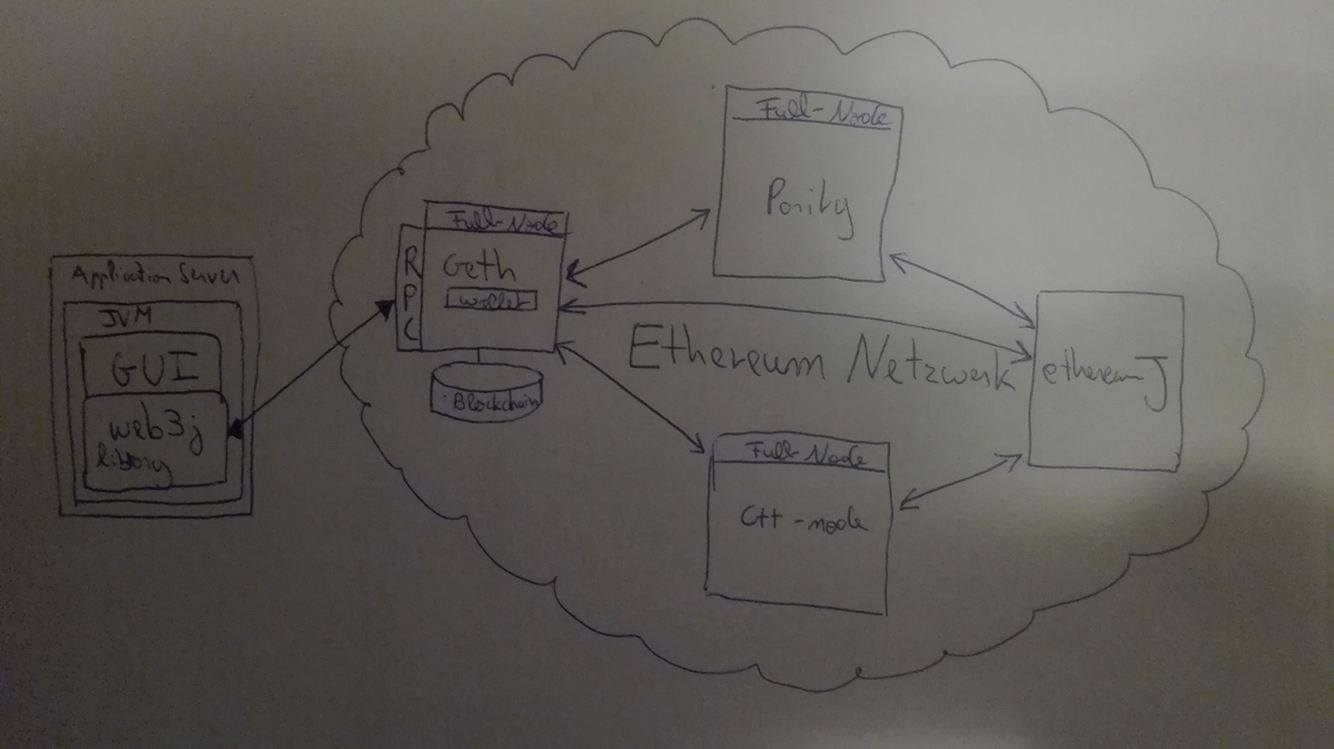
\includegraphics[width=1\linewidth]{Figures/ethereum_integration}
\decoRule
\caption{Ethereum: Netzwerk Integration}
\label{fig:ethereum_integration}
\end{figure}


\subsection{Smart Contract}
Die folgenden Codestücke beschreiben den TrustlessGambling Smart Contracts in der Sprache Solidity.
\subsubsection{Datenmodell}

\begin{lstlisting}[basicstyle=\small]
pragma solidity ^0.4.0;
contract TrustlessGambling {
    // constants
    uint8 public constant NBR_OF_SLOTS =3;
    uint public constant EXPECTED_POT_AMOUNT=1000;// WEI
    uint8 public constant PAYOUT_BLOCK_OFFSET =1;    
    // pot values
    uint public nbrOfParticipants;
    address[NBR_OF_SLOTS] public depositAddresses;
    address[NBR_OF_SLOTS] public payoutAddresses;
    uint public closingBlockNumber;
    uint public payoutBlockNumber;
    bytes32 public payoutBlockHash;
    uint public winner; // 0 -> NBR_OF_SLOTS-1
    bool public potClosed;
    uint public nbrOfMissedPayouts;
    // constructor
    function TrustlessGambling() public {
        nbrOfParticipants = 0;
        potClosed = false;
        nbrOfMissedPayouts = 0;
    }
}
\end{lstlisting}



\subsubsection{Einzahlungen}

\begin{lstlisting}
function deposit() payable public {
    deposit(msg.sender);
}
function deposit(address _payout) payable public {
    assert(msg.value == EXPECTED_POT_AMOUNT);
    assert(!potClosed);
    depositAddresses[nbrOfParticipants] = msg.sender;
    payoutAddresses[nbrOfParticipants] = _payout;
    nbrOfParticipants++;
    if (nbrOfParticipants == NBR_OF_SLOTS){
        closingBlockNumber = block.number;
        payoutBlockNumber = closingBlockNumber + PAYOUT_BLOCK_OFFSET;
        potClosed = true;
    }
}
\end{lstlisting}



\subsubsection{Auszahlungen}

\begin{lstlisting}[basicstyle=\small]
function payout() public{
    assert(potClosed);
    assert(block.number>payoutBlockNumber);
    payoutBlockHash = block.blockhash(payoutBlockNumber); 
    if(payoutBlockHash == 0){
        nbrOfMissedPayouts++;
    }else{
        winner = uint256(payoutBlockHash) % NBR_OF_SLOTS;
        address winnerAddress = payoutAddresses[winner];
        uint amount= EXPECTED_POT_AMOUNT*NBR_OF_SLOTS;
        amount += EXPECTED_POT_AMOUNT*NBR_OF_SLOTS*nbrOfMissedPayouts;
        winnerAddress.transfer(amount); // send pot amount to winner
        nbrOfMissedPayouts = 0;
    }
    potClosed = false;
    nbrOfParticipants=0;
}
\end{lstlisting}



\subsubsection{Einschränkungen}

Da man bei Ethereum im Conrtact Code nur auf die 256 letzten Blockheader zugreifen kann, unterscheidet sich der Smart Contract leicht von dem im Konzept beschriebenen.

\begin{figure}[H]
\centering
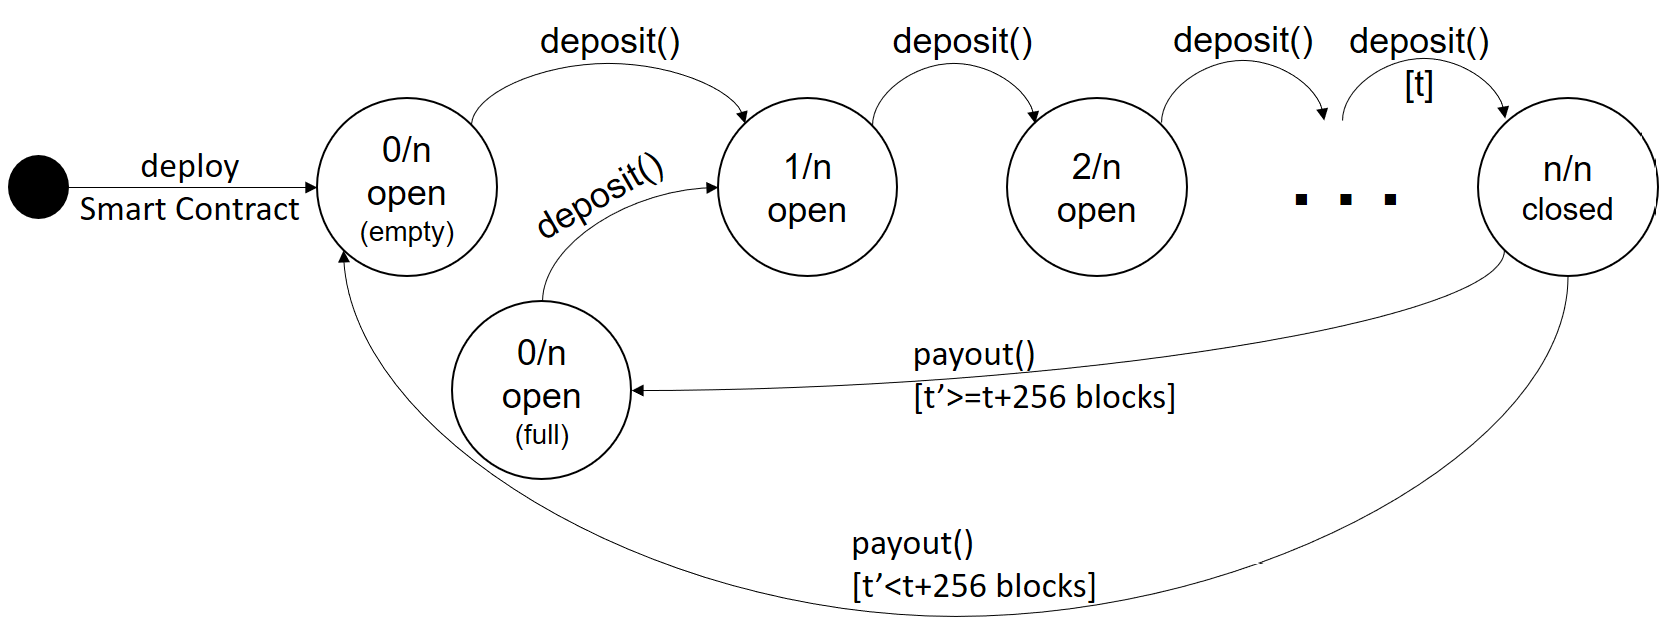
\includegraphics[width=1\linewidth]{Figures/umsetzung_eth/smart_contract_automat}
\decoRule
\caption{Smart Contract Umsetzung}
\label{fig:smart_contract_automat}
\end{figure}

\subsection{Smart Contract Bereitstellung}
Nachdem man den Smart Contract programmiert hat, muss man ihn zu Bytecode kompilieren und anschließen in einer Transaktion an das Ethereum Netzwerk senden. Dazu kann man die von Web3J bereitgestellten Comandline Tool nutzen. Dieses Tool hilft bei der Generierung einer Wallet und erlaubt es aus dem Contract Code eine Java Klasse zu generieren. Dieser Klasse ermöglicht die Interaktion mit dem Smart Contract. 

\begin{lstlisting}[basicstyle=\small]
public void createContract() throws Exception {
  String WALLET_FILENAME = "ethereum.json";
  String WALLET_PASSWORD = "changeit";
  long GAS_LIMIT = 1000000;
  ClassLoader classLoader = getClass().getClassLoader();
  File walletFile = new File(classLoader.getResource(WALLET_FILENAME).getFile());
  Credentials credentials = WalletUtils.loadCredentials(WALLET_PASSWORD, walletFile.getAbsolutePath());
  System.out.println("Account address = " + credentials.getAddress());
  Web3j web3j = Web3j.build(new InfuraHttpService("https://rinkeby.infura.io/" + UserConfiguration.API_KEY));
  BigInteger currentGasPrice = web3j.ethGasPrice().send().getGasPrice();
  TrustlessGambling contract = TrustlessGambling.deploy(web3j, credentials, currentGasPrice, BigInteger.valueOf(GAS_LIMIT)).send();
  String status = contract.getTransactionReceipt().get().getStatus();
  if ("0x1".equals(status)) {
    String address = contract.getContractAddress();
    System.out.println("Contract address = " + address);
    System.out.println("TXN hash = " + contract.getTransactionReceipt().get().getTransactionHash());
    System.out.println("Gas used = " + contract.getTransactionReceipt().get().getGasUsed());
  } else {
    System.out.println("Smart contract could not be deployed.");
  }
}
\end{lstlisting}
Die Ausführung des oben gezeigten Java Codes führt zu der folgenden Ausgabe:

\begin{lstlisting}
Account address = 0x2201f3919589b519135ce977cc0906c9481069b2
Contract address = 0x25c3136145fbd7f3b9217e58e2fabe3eb1928705
TXN hash = 0x06dce3c460b4caa595c5cc0f81ac78e7c70eeb1e89d3e0e6a017ea88e60dbce1
Gas used = 825846
\end{lstlisting}

In einem Blockchain Explorer kann man die Details der vom Full Node erstellten Transaktion\footnote{\url{https://rinkeby.etherscan.io/tx/0x06dce3c460b4caa595c5cc0f81ac78e7c70eeb1e89d3e0e6a017ea88e60dbce1}} und den kompilierten Contract Code\footnote{\url{https://rinkeby.etherscan.io/address/0x25c3136145fbd7f3b9217e58e2fabe3eb1928705\#code}} anschauen.
Alternativ zu Web3J lässt sich der Contract Code mithilfe eines Online Compilers \footnote{\url{https://ethereum.github.io/browser-solidity}} kompilieren und mithilfe des Ethereum Clients namens Mist\footnote{\url{https://github.com/ethereum/mist}} veröffentlichen.

\subsection{Geschäftslogik Webanwendung}

Dieses Kapitel zeigt, wie man in Etherem über einen Full Node mit dem Netzwerk interagieren kann. Die Webanwendung zeigt lediglich lediglich den aktuellen Zustand des Smart Contracts an. Die gesamte Geschäftslogik des Smart Contracts wird vom Etherem Netzwerk ausgeführt. Sollte die Webanwendung aufgrund  technischer Fehler ausfallen, hat dies keinerlei Auswirkung auf das eigentliche Spiel.

TODO 

\iffalse
\begin{enumerate}
\item Es gibt sowohl test als auch mainnet. Unterscheiden sih nur leicht durch protokoll und port. Teil sehen adressen anders aus. Bei ethereum creiert man sich ein wallet und die adresse ist für beide netzwerke gültig.
\item Auf dem testents gibts faucts für entwickler, die einem ein wenig testnet cryptowährung überweisen nachdem man ein captcha gelöst hat. Problem öffters mal down.
\item Bei ethereum hatte ich das typische Java problem, dass die web3jlib eine neuere verion vewendete als der Jboss Wildfly. Daher musste ich den jboss hochziehen
\item Neuer wildfly benutzt port /127.0.0.1:9990 den auch ein nvidea network service verwendet. den musste ich dann erst abschiessen.
\end{enumerate}
\fi

\subsection{Grafische Benutzeroberfläche}


Die Webapplikation konsumiert den lokal laufenden Webservice. Hier dann mal schauen wie viel schneller es ist die buisness logic direkt aufzurufen und den Webservice zu umgehen. Die Resultate ebenfalls in die Masterarbeit aufnehmen.

    Hier das Model View Controller Pattern verwenden.
    Tapestry Wen Framework erklären
    GUI Schicht ist es egal ob sie Ethereum Daten oder DASH Daten bekommt. Stichwort Tapestry Service.
    Bild von MVC pattern und java Klassendiagramm
    Zeigen wie die Empfangsaddresse in den QR code kodiert ist. Hier könnte man auch das entsprechende BIP nennen.
